\documentclass[a4paper]{article}

%% Language and font encodings
\usepackage[english]{babel}
\usepackage[utf8x]{inputenc}
\usepackage[T1]{fontenc}

%% Sets page size and margins
\usepackage[a4paper,top=3cm,bottom=2cm,left=3cm,right=3cm,marginparwidth=1.75cm]{geometry}

%% Useful packages
\usepackage{amsmath}
\usepackage{graphicx}
\usepackage[colorinlistoftodos]{todonotes}
\usepackage[colorlinks=true, allcolors=blue]{hyperref}
\usepackage{subfigure}
\usepackage{caption}
\usepackage{amsfonts}
\usepackage{amsthm}
\usepackage{upquote}
\usepackage{listings}
\usepackage{enumitem}
\usepackage{dirtytalk}
\usepackage{hyperref}
\usepackage{float}

\def\therefore{\boldsymbol{\text{ }
\leavevmode
\lower0.4ex\hbox{$\cdot$}
\kern-.5em\raise0.7ex\hbox{$\cdot$}
\kern-0.55em\lower0.4ex\hbox{$\cdot$}
\thinspace\text{ }}}

\title{Generating lecture notes out of a lecture video}
\author{CSED Sung Haebin 20160463}

\begin{document}
\maketitle
\section{Summary}
This project is about generating lecture notes out of a lecture video.
The goal is to recover images of a board scene, recovering the parts of the board that the lecturer occluded.

\section{Motivation}
Sometimes, when you watch a lecture video, it is painful to write lecture notes. 
If we automatically generate lecture notes, then it would definitely be convenient.
There are some situations that you could not see the full board because the lecturer is blocking it.
\begin{figure}[H]
\centering
\subfigure[human moving around the same board image, blocking the board 1]
{
    \label{fig:subfig1}
    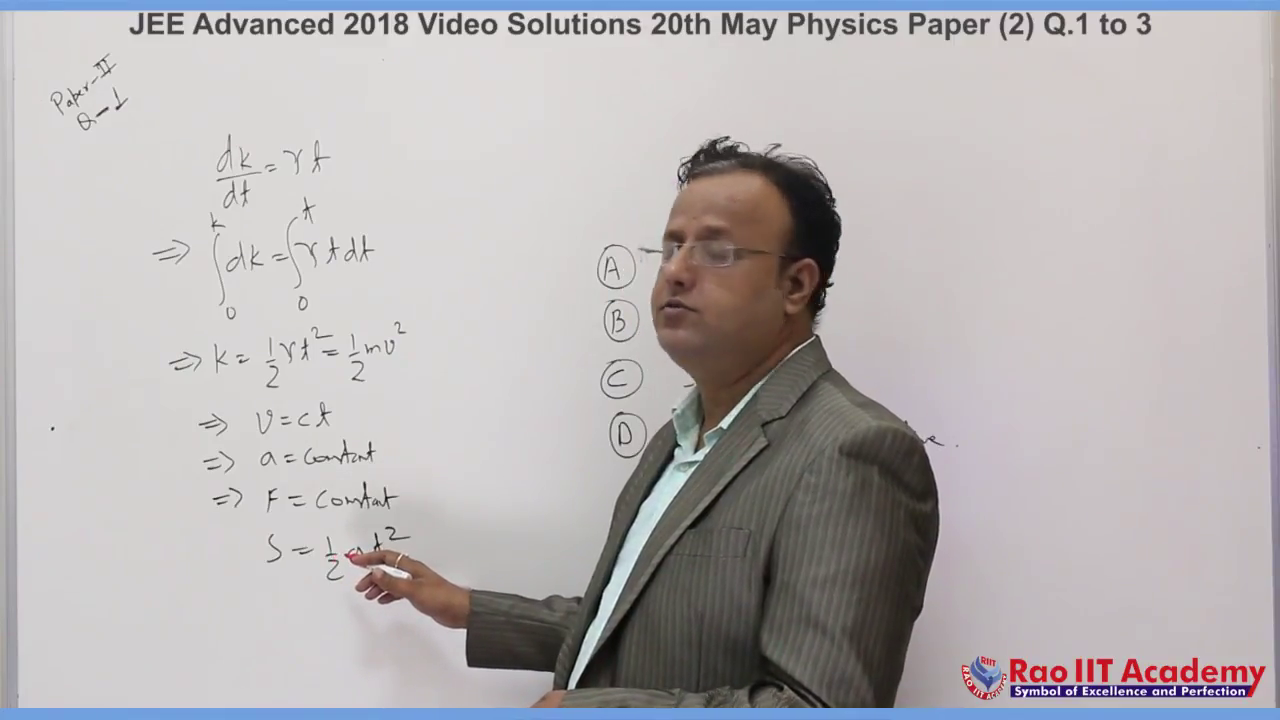
\includegraphics[scale=0.3]{2740.png}
}
\end{figure}
\begin{figure}[H]
\centering
\subfigure[human moving around the same board image, blocking the board 2]
{
    \label{fig:subfig2}
    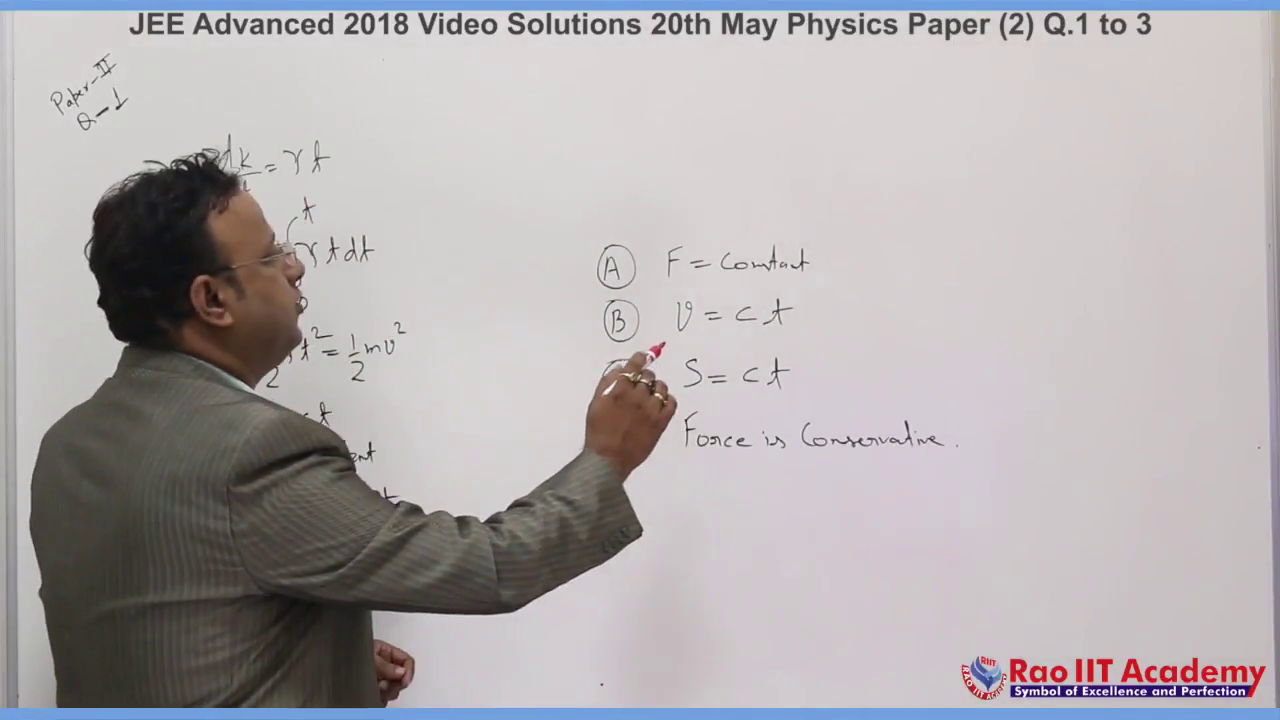
\includegraphics[scale=0.3]{2877.png}
}
\end{figure}

\section{Goals}
\subsection{Board Detection and Extracting Human Pixel}
We first have to know where the board is, to generate a picture of the board. Even if the camera is not looking at the board orthogonally, it's no problem, because we could calculate the homography matrix since we know that the board is rectangular. Then we have to extract the human(lecturer) part of a board to get rid of it. The most essential part of this project is to know whether a human is blocking the board or not, since we want to get rid of the human pixel.
\subsection{Board Transition Detection}
When do we have to take a snapshot? I would guess when it's when a lecturer erases the board, or when it moves to a new board, or when the board changes. I call this as a 'board transition'. This part is the most hardest part, because every lecture has different transitions with different magnitude, and it's hard to catch them all. For example, what if the lecturer erases only part of the board, and keeps going on? It is quite a task to detect them significantly.
\subsection{Board Recovery}
We now know the timing when we need to extract board images, so we recover the board in that time interval. We need to use a scheme to effectively predict the best board image possible, which is probably the latest shot of the board.
\subsection{(Optional) Making images to a pdf file}
A lecture note is best if it exists as a pdf, since a bunch of images are rather uncomfortable to keep.

\section{Implementation}
\subsection{Development Environment and Dataset}
In this project, I used python with opencv, PIL, numpy for image and video manipulation, and mxnet and gluoncv for semantic segmentation. \\
The goal was to make an application that could apply in general lecture videos, but soon I found that it was quite hard to achieve, especially in the difference of board transition. Instead, I found some lecture channel on Youtube, Rao IIT Academy(\url{https://www.youtube.com/user/raoiitacademy}), that had similar formats in every lecture. They always had a fixed camera with a full background board, with a quite explicit board transition by fading. So we could skip board detection, because the board is just a background. For this project, my target was only this channel's lectures, but I would always want to do some more and develop this program for more general use, if I have time later on.
\subsection{Human Exclusion by Semantic Segmentation}
Do we have to detect a human object? Well, if we could find out the color of the board and the color of the marker, then it might be possible to exclude colors that are not one of those to exclude obstacles. But this method is bad in some situations where the color of a person could be same of a board or marker, and it is quite hard to know the color of the markers. Then we might use object detection in detecting human with a bounding box. But in this case, a bounding box is too rough to effectively recover the board, so I decided to use semantic segmentation, which could effectively sort out the pixels of a human. I tried a few famous pretrained models, and found out that the best one for my case is Deeplabv3 with ResNet-152 as backbone network, trained on PASCAL VOC 2012, which has a 86.69 mIoU score.\cite{c1}
\begin{figure}[H]
\centering
\subfigure[result of semantic segmentation]
{
    \label{fig:subfig3}
    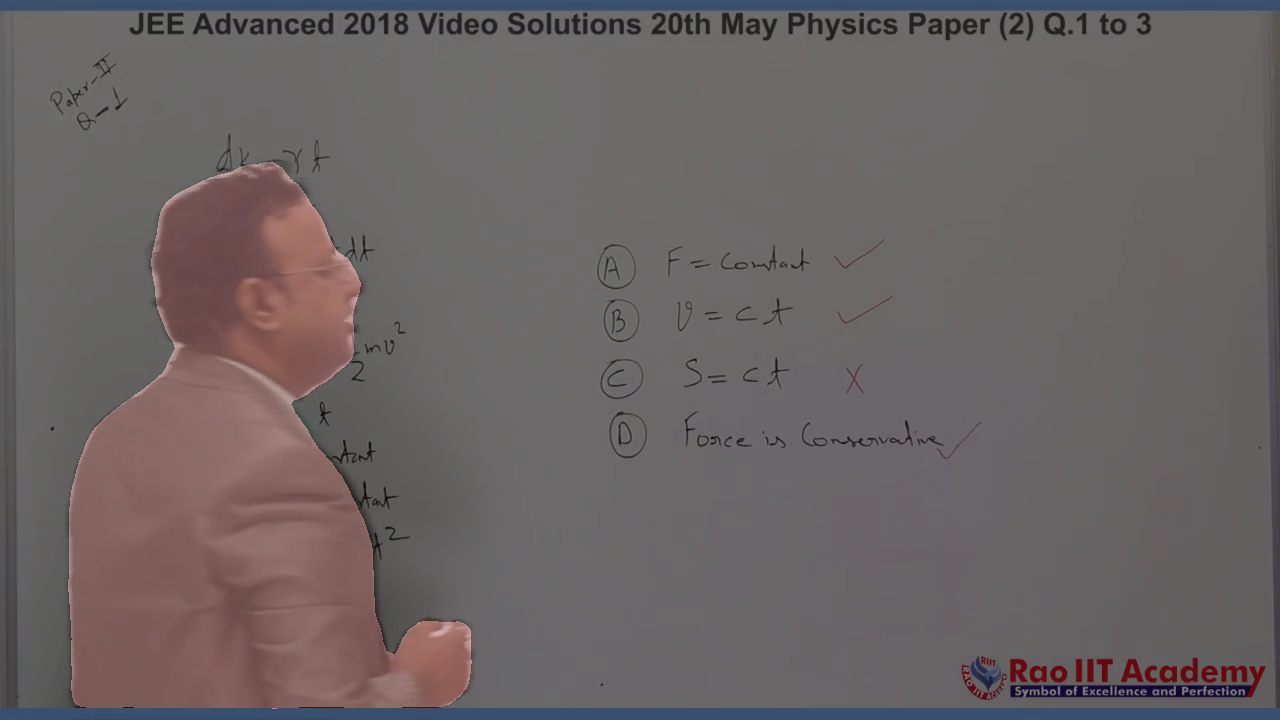
\includegraphics[scale=0.3]{3097_overlay.png}
}
\end{figure}
\subsection{Board Transition Detection}
This is the trickiest part. Even though I selected a very easy lecture format with explicit transition, my program still doesn't accurately extract the transitions. In this lecture, board transition is usually expressed with fading screens, so I calculated the euclidian distance of a white screen. Then by the change of the distance, if the distance decreases and increases, I thought of that as a transition time. The intervals(the amount of pages that I am going to produce) are made by having those transition times as endpoints. One thing you should keep in mind is, this algorithm is not only catching fading effects, and is not only limited to this dataset. If we erase a board, then the euclidian distance to the board color decreases, and increases when we rewrite. So we could apply this same metric in general cases, too. But this metric has its own problems, too; the whiteness distance could change just by the moving of a lecturer, since the coverage of a board changes, leading to distance change. I tried some tweaks to prevent getting these situations as a transition, but could not prevent them all.
\subsection{Board Recovery}
This is done by a simple algorithm, highly dependent on the board transition detection. We assume that all the board erasing movement is captured by board transition detection, so the interval we have only consists of drawing in the board augmentatively. So we start from the last frame of the interval, and we rewind the frame with a particular stride, and check if the pixel obstructed in the future frame is visible on the previous frame. If the recovery reaches 100 percent, we stop the rewind and move on to the next interval. This algorithm itself is quite descent, but if the transition detection is inaccurate or too sensitive, then it could lead to weakly-merged board images.
\begin{figure}[H]
\centering
\subfigure[result of board recovery]
{
    \label{fig:subfig3}
    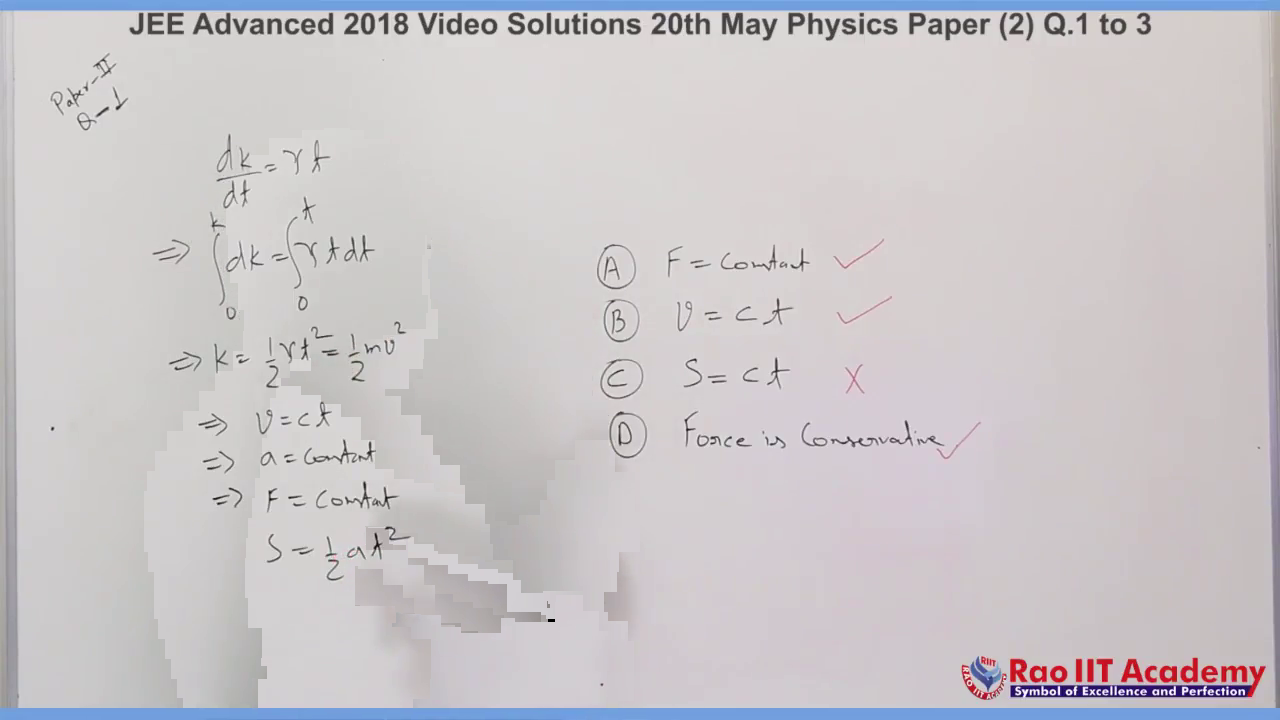
\includegraphics[scale=0.3]{1529_3278.png}
}
\end{figure}
\subsection{Gathering images to a pdf file}
This is just done by using fpdf, a pdf library.


\section{Notable References}
\subsection{Deeplabv3\cite{c2}}
This model is also introduced in our lecture. It uses Atrous convolution and post processing. It is one of the state-of-the-art models in semantic segmentation.


\section{Gallery}
\begin{figure}[H]
\centering
\subfigure[some results of board recovery]
{
    \label{fig:subfig4}
    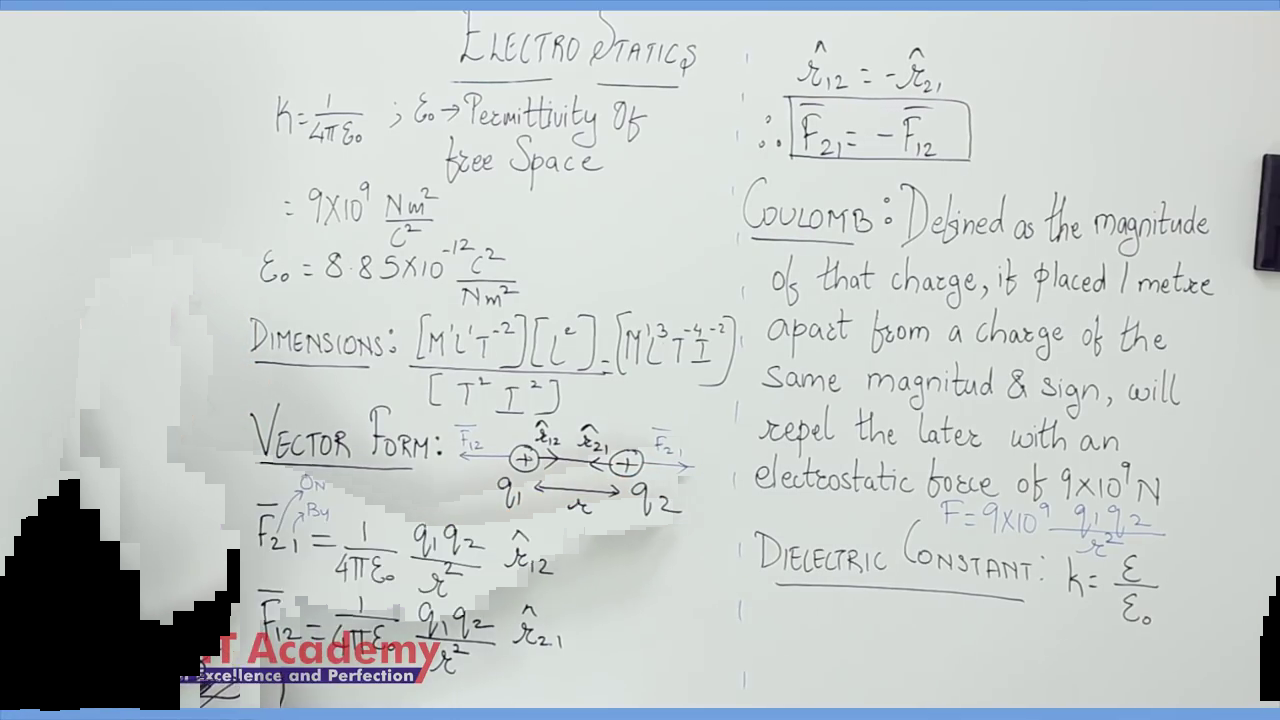
\includegraphics[scale=0.3]{19477_20525.png}
}
\end{figure}

\section{Discussion}
\begin{description}[style=nextline]
\item[How could we make semantic segmentation more accurate?]
This pretrained model itself has some decent performance, but it rarely omits some body parts. This could be done by fine tuning the model. I skipped fine tuning in this project because I didn't have much time to create the labels for the lecture images. But these particular videos are quite easy in that they have a similar structure and camera view, so it wouldn't be that hard to achieve good results in this particular dataset.
\item[How could we make board transition detection more accurate?]
I thought about some several schemes to achieve accurate board transition detection, but it is quite tricky. First, I thought of blur detection, since in this dataset, a fade occurs, and this causes blurring. So we could calculate the variance of laplacian to detect blurriness, but this is a video, so blurring commonly happens, even when it's not fading. Or we could just calculate the euclidian difference between the adjacent frames of the board, and also calculate how much pixels the color of the board was covered to detect erasing events. I think this could be an effective metric, but these pixel color-specific metrics usually happen to fail, since this is a video, can color changes frequently in the video even it is the same color in reality.
\item[How could we make recover boards more smoothly?]
As you see in the results, the pixel colors actually tend to change a little bit during the video, leading to uncontinuous pixel color results of recovery. This could be solved by some interpolation or some heuristic to equalize the colors, but I did not implement those schemes yet.
\end{description}

\begin{thebibliography}{1}
\bibitem{c1}PASCAL VOC Challenge performance evaluation of my pretrained model : \url{http://host.robots.ox.ac.uk:8080/anonymous/XZEXL2.html}
\bibitem{c2}Chen, Liang-Chieh, et al. “Rethinking atrous convolution for semantic image segmentation.” arXiv preprint arXiv:1706.05587 (2017). : \url{https://arxiv.org/abs/1706.05587}
\end{thebibliography}

\end{document}
